\section{Introduktion}
Netværklaget omhandler en host-to-host kommunikation service dvs. dens opgave består i at sende pakker fra en ‘sending host’ til en ‘receiving host’.
\begin{center}
  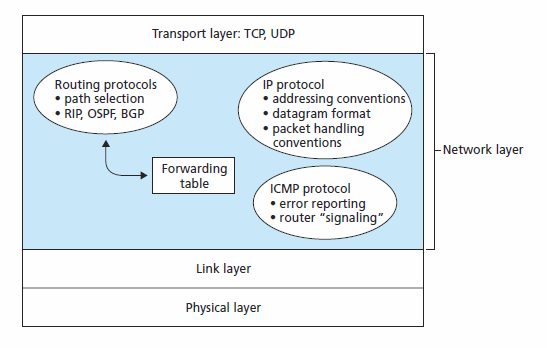
\includegraphics{4-network-layer/networklayer.png}
\end{center}
\begin{itemize}
	\item Står for addressering
	\item Leverer pakker til applikationer.
	\item Routing
	\item Forwarding 
	\item Modtager segmenter fra transportlag -> indkapsler dette i datagram (+IP) -> Videre til routeren.
\end{itemize}

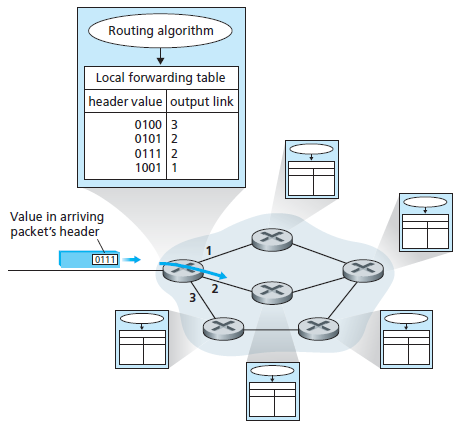
\includegraphics{4-network-layer/RoutingForwardring.png}

\subsection{Forwarding}
\begin{itemize}
\item Ankommen pakke i router skal flyttes til udgående link (Videre på netværk/Tilkoblet klient på router)
\item Forwardring tabel
\item Analyserer bestemt field (header).
\item Bruges til at indeksere i forwarding tabel.
\end{itemize}

\subsection{Routing}
\begin{itemize}
\item Finde vej ved hjælp af routing protokoller.
\item Stibestemmelse
\item Routing Algoritmer
\end{itemize}

\section{Services på netværkslaget}
\begin{itemize}
\item Guaranteed delivery (Garanti for pakkes ankomst ved destination) + bounded delay.
\item In-order-packet-delivery (Ankommer i rækkefølgen de blev sendt).
\item Security Services (Kryptering af datagrammer)
\item Osv.
\end{itemize}

\section{Virtuelle kredsløb og datagramnetværk}
\subsection{Virtuelle kredsløb}
{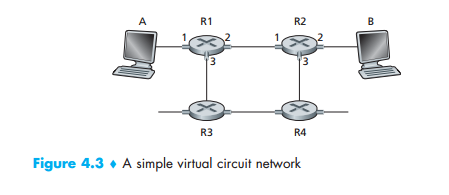
\includegraphics{4-network-layer/vc-network.png}
\begin{itemize}
	\item 1) Rute (En række routere og links). 
	\item 2) VC-nummer (Ét nummer for hver link langs en rute)
	\item 3) Indgange i FW-table i hver router land en Route
	\item Videresendelsestabel
	\item Opbevarer oplysninger om forbindelsesstatus.
\end{itemize}

\subsection{Datagramnetværk}
{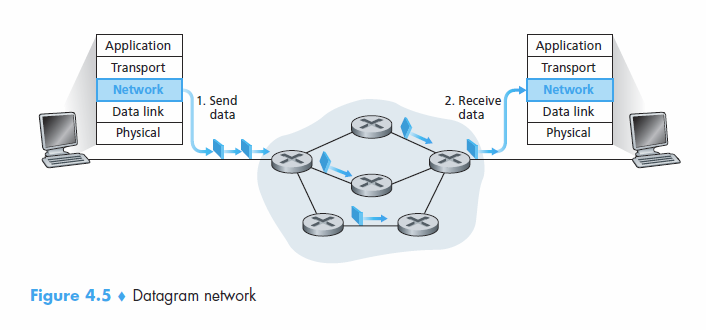
\includegraphics{4-network-layer/datagramnetwork.png}
\begin{itemize}
	\item For hver packetforsendelse - destinations adresse tilføjes og afsendes.
	\item Packet bevæger sig igennem routere mod distination.
	\item Routerne benytter destinationsadressen til at forward. 
	\item Opbevarer INGEN oplysninger om forbindelsesstatus
	\item 32 bit destinationsadresse (IP-Datagram).
\end{itemize}

\section{Sådan virker en router}
En router er en enhed på et computernetværk som forbinder et antal logiske eller fysiske netværk ved at videresende pakker fra et netværk til deres destination på et andet netværk i en process kaldet routing. Routeren arbejder på OSI-modellens lag 3 (netværkslaget), i internetprotokollen kaldes dette lag IP-laget.
\begin{center}
  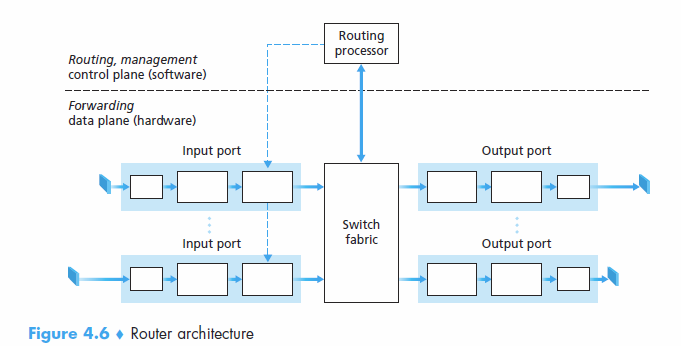
\includegraphics[scale=0.8]{4-network-layer/whats-inside-a-router.png}
\end{center}
\begin{itemize}
	\item Input porte (lookup function - skal en packet sendes igennem denne?)
	\item Switching fabric (Forbinder input/ output porte)
	\item Output porte (Herfra sendes packets - Bidirectional) 
	\item Routing processor (Routing protokoller / states på links)
\end{itemize}


{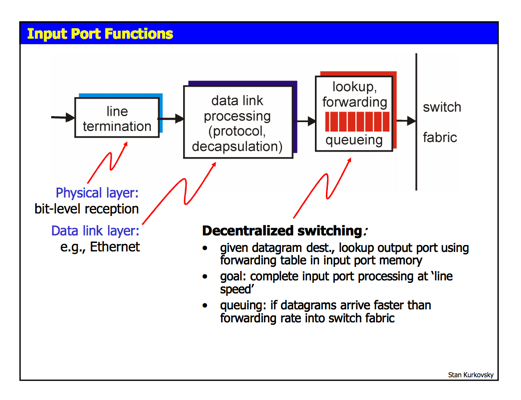
\includegraphics{4-network-layer/router-input-port}
{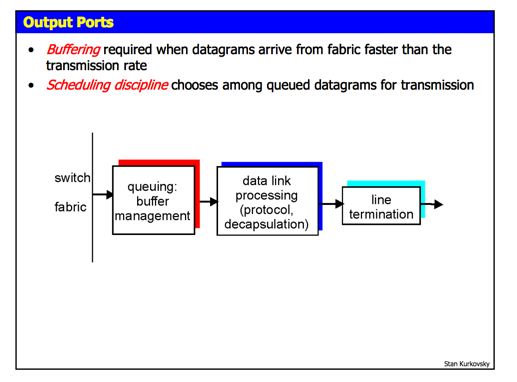
\includegraphics{4-network-layer/router-output-port.png}

\section{Internetprotokollen – IP}
Den protokol der bruges på internettets netværkslag er IP protokollen. 
Derfor kaldes internettets netværkslag også for IP-laget. Internetprotokollen er imidlertid bare en del af internettets netværkslag, der består af 3 hovedkomponenter.
\begin{center}
  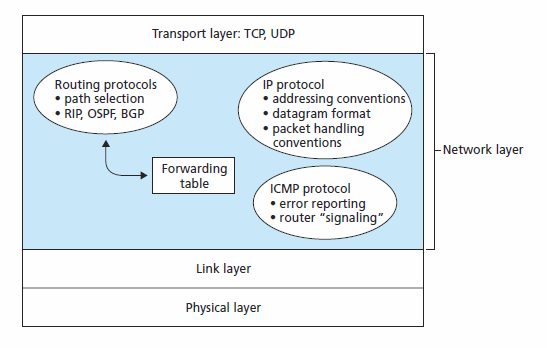
\includegraphics{4-network-layer/networklayer.png}
\end{center}
\begin{itemize}
	\item Internet Protocol(adressering - felter i datagrammet - IPv4 - IPv6)
	\item Stibestemmelse(beregne pakkes sti - vedligeholdelse af netværket)
	\item Fejlrapportering(rapportere  fejl i datagrammet - ICMP
\end{itemize}

\section{Ipv4 datagram}
{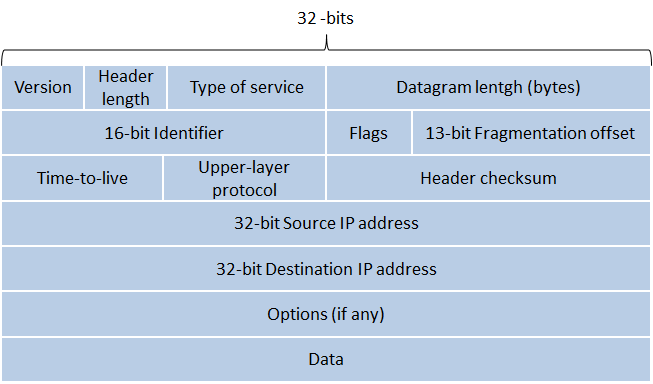
\includegraphics{4-network-layer/IPv4_datagram.png}
\begin{itemize}
	\item Version: (IPv4 / IPv6)
	\item Header length: (Hvor starter dataen?)
	\item Servicetype: (IP-datagram type: Realtime / non-realtime.)
	\item Datagram-length: Datagrammets længde (Header + data)
	\item Identifikation, flag og start på opdeling.
	\item Time-to-live: (Sørger for at datagram ikke lever for evig - counter dekrementeres).
	\item Protokol: TCP eller UDP på transportlag.
	\item Header checksum: Udregnes fra summen af bytes - kontrolleres af modtager.
	\item Source/destination IP address: Afsender og modtageradresse (IP)
	\item Settings: Mulighed for udvidelse af IP header.
	\item Data: Transportlag segmentet (Reel data).
\end{itemize}

\section{IPv4 adressering}
En vært er sædvanligvis koblet til netværket med én forbindelse. Grænsen mellem værten og det fysiske netværk kaldes en interface.
\begin{center}
  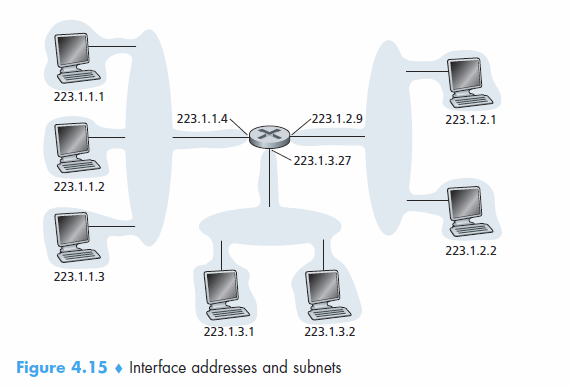
\includegraphics{4-network-layer/ipv4-adressering.png}
\end{center}
\begin{itemize}
	\item Interface (Router har et interface for hvert link.)
 	\item Hvert host og router interface har en IP tilknyttet.
	\item IP adressen knyttet til interfacet
	\item IP addresse 32 bits, dotted decimal format
	\item Flere host interfaces på ét router interface = subnet.
	\item 223.1.1.0/24 - /24 notation = subnet mask.
\end{itemize}

  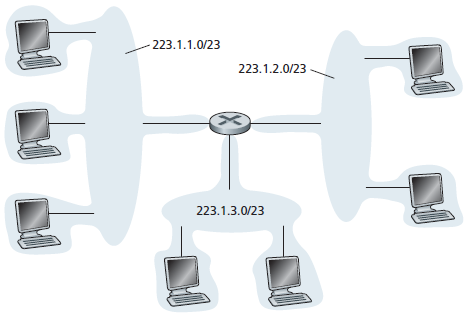
\includegraphics{4-network-layer/ivpsubnet.png}

\section{Hierarkisk routing}
En router er en enhed på et computernetværk som forbinder et antal logiske eller fysiske netværk ved at videresende pakker fra et netværk til deres destination på et andet netværk i en process kaldet routing. Routeren arbejder på OSI-modellens lag 3 (netværkslaget), i internetprotokollen kaldes dette lag IP-laget.
\begin{center}
  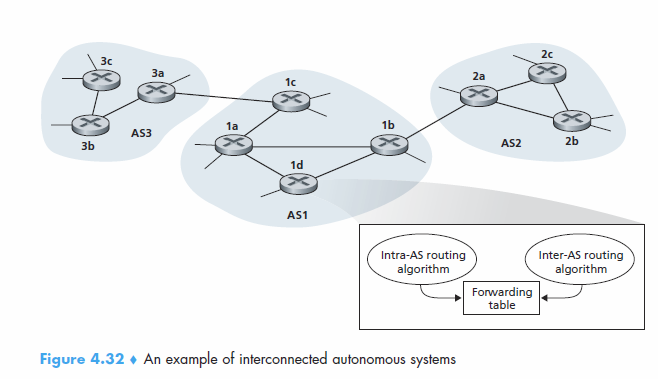
\includegraphics[scale=0.8]{4-network-layer/hierarkisk-routing.png}
\end{center}
\begin{itemize}
	\item Metode til at route i netværk.
	\item Baseret på hierarkisk adressering.
	\item Arrangering af routere i et hierarki. 
\end{itemize}


\section{Tildeling af IP adresser}
\begin{itemize}
	\item Manuel konfiguration
	\item Dynamic Host Configuration Protocol – DHCP(plug-and-play protokol - flere brugere - færre ip adresser - let at administrerer - adressekonflikt)
\end{itemize}


\section{ICMP – Internet Control Message Protocol}
\begin{itemize}
	\item Error reporting
	\item Hvis "Destination network unreachable" fejl modtages = IMCP.
	\item Sti til host kunne ikke findes.
	\item Betragtes som en del af IP - men befinder sig lige over IP.
	\item ICMP beskeder sender i IP datagrammer.
	\item ICMP = IP Payload, ligesom UDP og TCP segmenter.

\end{itemize}
{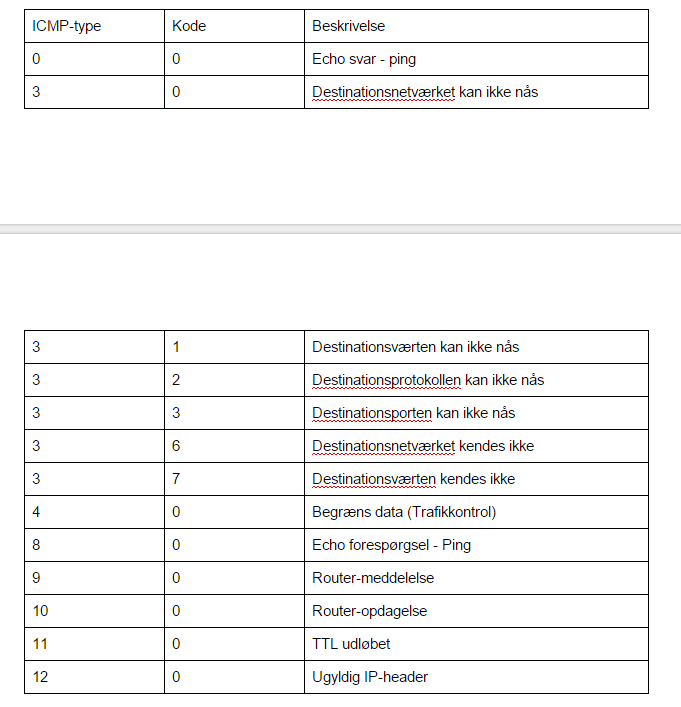
\includegraphics{4-network-layer/icmp-tabel.png}

